\documentclass[fontsize=12pt,
               paper=a4,
               twoside=false,
               parskip=half,
               ]{scrartcl}

% Load the packages
% Packages Template
% =================
% 
% Contains packages used for project documentation
% 
% @author burgc5
% 
% To use this simply enter: % Packages Template
% =================
% 
% Contains packages used for project documentation
% 
% @author burgc5
% 
% To use this simply enter: % Packages Template
% =================
% 
% Contains packages used for project documentation
% 
% @author burgc5
% 
% To use this simply enter: \input{./packages.tex}

\usepackage[utf8]{inputenc}
\usepackage[T1]{fontenc}

% Set font to latin modern
\usepackage{lmodern}

\usepackage[pdftex]{graphicx}
\usepackage{epstopdf}

% Create links in pdf documents
\usepackage[colorlinks,pdfpagelabels,pdfstartview=FitH,bookmarksopen=true,bookmarksnumbered=true,linkcolor=black,plainpages=false,hypertexnames=false,citecolor=black] {hyperref}
\hypersetup{
    colorlinks,%
    citecolor=black,%
    filecolor=black,%
    linkcolor=black,%
    urlcolor=black
}
\urlstyle{same}

% Use \enquote{} to create quotation marks
\usepackage{csquotes}

% Create professional tables with booktabs
% @see http://en.wikibooks.org/wiki/LaTeX/Tables#Professional_tables
\usepackage{booktabs}

% Customizable enumerates/itemizes
\usepackage{enumitem}

% SVN meta information
\usepackage{svn}


\usepackage[utf8]{inputenc}
\usepackage[T1]{fontenc}

% Set font to latin modern
\usepackage{lmodern}

\usepackage[pdftex]{graphicx}
\usepackage{epstopdf}

% Create links in pdf documents
\usepackage[colorlinks,pdfpagelabels,pdfstartview=FitH,bookmarksopen=true,bookmarksnumbered=true,linkcolor=black,plainpages=false,hypertexnames=false,citecolor=black] {hyperref}
\hypersetup{
    colorlinks,%
    citecolor=black,%
    filecolor=black,%
    linkcolor=black,%
    urlcolor=black
}
\urlstyle{same}

% Use \enquote{} to create quotation marks
\usepackage{csquotes}

% Create professional tables with booktabs
% @see http://en.wikibooks.org/wiki/LaTeX/Tables#Professional_tables
\usepackage{booktabs}

% Customizable enumerates/itemizes
\usepackage{enumitem}

% SVN meta information
\usepackage{svn}


\usepackage[utf8]{inputenc}
\usepackage[T1]{fontenc}

% Set font to latin modern
\usepackage{lmodern}

\usepackage[pdftex]{graphicx}
\usepackage{epstopdf}

% Create links in pdf documents
\usepackage[colorlinks,pdfpagelabels,pdfstartview=FitH,bookmarksopen=true,bookmarksnumbered=true,linkcolor=black,plainpages=false,hypertexnames=false,citecolor=black] {hyperref}
\hypersetup{
    colorlinks,%
    citecolor=black,%
    filecolor=black,%
    linkcolor=black,%
    urlcolor=black
}
\urlstyle{same}

% Use \enquote{} to create quotation marks
\usepackage{csquotes}

% Create professional tables with booktabs
% @see http://en.wikibooks.org/wiki/LaTeX/Tables#Professional_tables
\usepackage{booktabs}

% Customizable enumerates/itemizes
\usepackage{enumitem}

% SVN meta information
\usepackage{svn}


% SVN Meta
\SVN $Date: 2012-05-11 14:51:38 +0200 (Fr, 11 Mai 2012) $
\SVN $Revision: 101 $
\SVN $HeadURL: https://svn.bfh.ch/repos/projects/patmon1/trunk/doc/src/use_case_model.tex $


\begin{document}

% Document title for title.tex
\newcommand{\doctitle}{Use Case Model}
% Titlepage Template
% ==================
% 
% @author burgc5
% 
% To use this simply enter: % Titlepage Template
% ==================
% 
% @author burgc5
% 
% To use this simply enter: % Titlepage Template
% ==================
% 
% @author burgc5
% 
% To use this simply enter: \input{./title.tex}
% 
% You have to define the commands '\doctitle' and '\docrevision' to give the 
% document a title and a revision on its titlepage.
% Do this with the following command:
% \newcommand{\doctitle}{Document title goes here}
%
% SVN:
% ----
% You also have to define the variables:
% \SVN $Date$
% \SVN $Revision$
%
% As executing the following command on the file:
% > svn propset svn:keywords "Date Revision" filename.tex
% 
% This titlepage needs:
% \usepackage[pdftex]{graphicx}
% \usepackage{svn}
%

\begin{titlepage}

\begin{center}

% Team-logo

\includegraphics[width=0.35\textwidth]{./comet-logo.eps}\\[2.5cm]    

% Project title
\textsc{\Large Comet Patient Monitor}\\[2cm]

% Document title
{ \huge \bfseries \doctitle{}}\\[3cm]

% Members/Client
\begin{minipage}{0.45\textwidth}
\begin{flushleft} \large
\emph{Team Members:}\\
Patrick \textsc{Haring}\\
Christian \textsc{Bürgi}
\end{flushleft}
\end{minipage}
\begin{minipage}{0.45\textwidth}
\begin{flushright} \large
\emph{Client:} \\
Prof.~Dr.~Olivier \textsc{Biberstein}\\
~
\end{flushright}
\end{minipage}

\vfill

{\large 
Revision: \SVNRevision \\[0.2cm]
\SVNDate \\[0.2cm]
{\footnotesize \itshape \url{\SVNHeadURL?p=\SVNRevision}}}

\end{center}

\end{titlepage}
% 
% You have to define the commands '\doctitle' and '\docrevision' to give the 
% document a title and a revision on its titlepage.
% Do this with the following command:
% \newcommand{\doctitle}{Document title goes here}
%
% SVN:
% ----
% You also have to define the variables:
% \SVN $Date$
% \SVN $Revision$
%
% As executing the following command on the file:
% > svn propset svn:keywords "Date Revision" filename.tex
% 
% This titlepage needs:
% \usepackage[pdftex]{graphicx}
% \usepackage{svn}
%

\begin{titlepage}

\begin{center}

% Team-logo

\includegraphics[width=0.35\textwidth]{./comet-logo.eps}\\[2.5cm]    

% Project title
\textsc{\Large Comet Patient Monitor}\\[2cm]

% Document title
{ \huge \bfseries \doctitle{}}\\[3cm]

% Members/Client
\begin{minipage}{0.45\textwidth}
\begin{flushleft} \large
\emph{Team Members:}\\
Patrick \textsc{Haring}\\
Christian \textsc{Bürgi}
\end{flushleft}
\end{minipage}
\begin{minipage}{0.45\textwidth}
\begin{flushright} \large
\emph{Client:} \\
Prof.~Dr.~Olivier \textsc{Biberstein}\\
~
\end{flushright}
\end{minipage}

\vfill

{\large 
Revision: \SVNRevision \\[0.2cm]
\SVNDate \\[0.2cm]
{\footnotesize \itshape \url{\SVNHeadURL?p=\SVNRevision}}}

\end{center}

\end{titlepage}
% 
% You have to define the commands '\doctitle' and '\docrevision' to give the 
% document a title and a revision on its titlepage.
% Do this with the following command:
% \newcommand{\doctitle}{Document title goes here}
%
% SVN:
% ----
% You also have to define the variables:
% \SVN $Date$
% \SVN $Revision$
%
% As executing the following command on the file:
% > svn propset svn:keywords "Date Revision" filename.tex
% 
% This titlepage needs:
% \usepackage[pdftex]{graphicx}
% \usepackage{svn}
%

\begin{titlepage}

\begin{center}

% Team-logo

\includegraphics[width=0.35\textwidth]{./comet-logo.eps}\\[2.5cm]    

% Project title
\textsc{\Large Comet Patient Monitor}\\[2cm]

% Document title
{ \huge \bfseries \doctitle{}}\\[3cm]

% Members/Client
\begin{minipage}{0.45\textwidth}
\begin{flushleft} \large
\emph{Team Members:}\\
Patrick \textsc{Haring}\\
Christian \textsc{Bürgi}
\end{flushleft}
\end{minipage}
\begin{minipage}{0.45\textwidth}
\begin{flushright} \large
\emph{Client:} \\
Prof.~Dr.~Olivier \textsc{Biberstein}\\
~
\end{flushright}
\end{minipage}

\vfill

{\large 
Revision: \SVNRevision \\[0.2cm]
\SVNDate \\[0.2cm]
{\footnotesize \itshape \url{\SVNHeadURL?p=\SVNRevision}}}

\end{center}

\end{titlepage}

\tableofcontents

%=======
% ACTORS
%=======

\section{Actors}

\subsection{List of actors}

\begin{tabular}{llp{9cm}}
\toprule
\textbf{Actor} & \textbf{Type} & \textbf{Description} \\ 
\midrule
\emph{Doctor} & primary & \emph{Doctor}s are employees of the hospital. They are specialists
in their domain but not as computer users. \emph{Doctor}s use the system as a tool
in daily work for monitoring \emph{patient}s. \\ 
\emph{Administrator} & primary & The \emph{administrator} is an employee of the hospital as
well. He is responsible for the hospital's IT systems to work. He configures
the system for the \emph{doctor}s to work with. He is not a \emph{doctor}. \\ 
\emph{OT-Logger} & supporting & The \emph{OT-Logger}s are devices which are used to monitor
\emph{patient}'s temperatures over a period of time. They can be remotely polled by 
the system. A device can only be reused after appliance on a \emph{patient} if the device was reset.\\ 
\emph{Patient} & off-stage & \emph{Patient}s have the monitoring device attached for a period from a few days to a few weeks. \\
\emph{Email-Server} & supporting & The \emph{email-server} will send the activation code for the first authentication of the \emph{doctor} against the server.

\\ 
\bottomrule 
\end{tabular} 

\subsection{Primary actor goals}

\begin{description}

\item[Doctor:] \hfill \\
A \emph{doctor} uses the system to assign a device to a \emph{patient} for an observation period. During the period and after it has ended, he consults the system to inspect the recorded data. After the observation period has completed he wants to reset the devices and prepare them thereby for reuse.

\item[Administrator:] \hfill \\
The \emph{administrator} wants to create and delete accounts for the \emph{doctor}s.

\end{description}

%==================
% Use cases (brief)
%==================


\section{Use cases (brief)}

\subsection{Doctor}

\begin{description}

\item[Assign device:] In order to start a monitoring period, the \emph{doctor} has to assign a monitoring device to the \emph{patient} in the system. The \emph{doctor} looks up the \emph{patient}'s profile. He chooses the option to assign a device to this \emph{patient}. He enters the device's data. The system checks, if the device is ready for assignment (i.e. that it is not assigned yet). Then he enters the monitoring period's parameters. The system configures the device and saves the configuration internally.

\item[Consult monitoring data:] As soon as the monitoring device reports data to the system, the \emph{doctor} is able to see a report of the data, which has been recorded so far. After the monitoring period has ended, he can consult a detailed report of the period.

\item[Reset device:] When a \emph{patient} returns his monitoring device, the \emph{doctor} has to reset the device. He enters the device's number and chooses it to be reset. This procedure is even possible if the monitoring period has not ended yet.

\item[Register patient:] For registering a \emph{patient} in the system the \emph{doctor} enters the \emph{patient}'s social security number. The system checks, if the \emph{patient} is already registered. If the \emph{patient} is not already in the system, the \emph{doctor} enters all the necessary data about the \emph{patient} and the system stores it internally.

\item[Authenticate against system:] The \emph{doctor} authenticates against the system by entering his email address and password. If his account is decativated, he has to enter the activation code he received by email. This procedure is necessary to verify the \emph{doctor}'s email address.

\end{description}

\subsection{Administrator}

\begin{description}

\item[Create account:] A new \emph{doctor} has to be registered in the system. The \emph{administrator} enters the \emph{doctor}'s name and mail address. The system presents the entered information. The \emph{administrator} verifies it and confirms that to the system. The system creates an account with a random initial password and presents after successful creation the full account data to the \emph{administrator}. He records the initial password which he has to give to the \emph{doctor} in person. There is also an email sent to the entered account email by using the \emph{email-server}. It contains an activation code, which is used by the \emph{doctor} for his first login.

\item[Delete account:] A \emph{doctor} has to be deleted from the system. The account can only be deleted if it was disabled (and not enabled again) for a given period. The \emph{administrator} archives the data of the \emph{patient}s, which are referenced to this account and deletes the \emph{doctor}'s account. By deleting a \emph{doctor}'s account the system also deletes all corresponding \emph{patient} data (in the system).

\item[Disable account:] An account of a \emph{doctor} has to be disabled. The \emph{administrator} disables the login of the \emph{doctor}. Thereby the account is also deactivated (when enabled again, the \emph{doctor} needs to reactivate the account). The system notifies the \emph{doctor} by means of an email via the \emph{email-server}. 

\item[Enable account:] A disabled account of a \emph{doctor} has to be enabled again. The System generates a new activation code and sends it via the \emph{email-server} to the \emph{doctor}. If necessary, he also resets the \emph{doctor}'s password.

\item[Reset password:] A \emph{doctor}'s password has to be changed. The \emph{administrator} generates a new password and gives it to the \emph{doctor} in person.

\item[Authenticate against System:] The \emph{administrator} authenticates against the system by entering his email address and password.

\end{description}

%==========================
% Use cases (fully-dressed)
%==========================

\section{Use cases (fully-dressed)}

% UC1
%----

\subsection{Use Case UC1: Assign device}

\textbf{\textsf{Scope:}} Comet Patient Monitor

\textbf{\textsf{Level:}} user goal

\textbf{\textsf{Primary actor:}} \emph{Doctor}

\textbf{\textsf{Preconditions:}} \emph{Doctor} is authenticated against the system. \emph{Patient} is registered in the System.

\textbf{\textsf{Postconditions:}} The monitoring device is assigned to the \emph{patient}. The device will monitor the temperature during a given period.

\textbf{\textsf{Main success scenario:}}

\begin{enumerate}[leftmargin=3em]
	\item \emph{Doctor} enters the \emph{patient}'s name and/or social security number into system.
	\item System looks up matching \emph{patient} profiles and displays them to the \emph{doctor}.
	\item \emph{Doctor} selects the appropriate \emph{patient} profile.
	\item System displays detailed version of the selected profile.
	\item \emph{Doctor} enters the device identification number into the system.
	\item System checks if the device is already assigned to a \emph{patient}.
	\item \emph{Doctor} enters the beginning and the end of the observation period into the system.
	\item System verifies that the entered data is a valid observation period.
	\item \emph{Doctor} enters the frequency by which the measures have to be performed.
	\item System configures the device.
	\item System saves assignment of the device to the \emph{patient}.
\end{enumerate}

\textbf{\textsf{Extensions:}}

\begin{itemize}[leftmargin=3em]
	\item[*a.] At any time, \emph{doctor} cancels assignment operation.
	\begin{enumerate}
		\item System discards all entered data.
	\end{enumerate}
	\item[2a.] No profile is found.
	\begin{enumerate}
		\item System signals error and reverts to step 1 in main scenario.
	\end{enumerate}
	\item[2b.] Correct \emph{patient} profile is not found.
	\begin{enumerate}
		\item \emph{Doctor} verifies entered data.
		\begin{itemize}
			\item[1a.] \emph{Patient} is not registered (violation of precondition!):
			\begin{enumerate}[label=\arabic*.]
				\item \emph{Doctor} cancels assignment operation and proceeds with UC4.
			\end{enumerate}
		\end{itemize}
		\item \emph{Doctor} proceeds with step 1 in main scenario.
	\end{enumerate}
	\item[4a.] \emph{Doctor} selected wrong \emph{patient} profile.
	\begin{enumerate}
		\item \emph{Doctor} cancels assignment to selected profile.
		\item System reverts to step 2 in main scenario.
	\end{enumerate}
	\item[6a.] Device is already assigned.
	\begin{enumerate}
		\item System signals error.
		\item \emph{Doctor} gets a different device.
		\item System reverts to step 5 in main scenario.
	\end{enumerate}
	\item[8a.] Invalid observation period.
	\begin{enumerate}
		\item System signals error and reverts to step 7 in main scenario.
	\end{enumerate}
	\item[10a.] Error while configuring the device.
	\begin{enumerate}
		\item System signals error.
		\item \emph{Doctor} marks device as faulty and sends it to reparation.
		\item \emph{Doctor} gets a different device.
		\item System reverts to step 5 in main scenario.
	\end{enumerate}
\end{itemize}

% UC2
%----

\subsection{Use Case UC2: Consult monitoring data}

\textbf{\textsf{Scope:}} Comet Patient Monitor

\textbf{\textsf{Level:}} user goal

\textbf{\textsf{Primary actor:}} \emph{Doctor}

\textbf{\textsf{Preconditions:}} \emph{Doctor} is authenticated against the system. \emph{Patient} is registered. There is monitored data in the system.

\textbf{\textsf{Postconditions:}} \emph{Doctor} has been presented a report over the monitored data.

\textbf{\textsf{Main success scenario:}}

\begin{enumerate}[leftmargin=3em]
	\item \emph{Doctor} enters the \emph{patient}'s name and/or social security number into system.
	\item System looks up matching \emph{patient} profiles and displays them to the \emph{doctor}.
	\item \emph{Doctor} selects the appropriate \emph{patient} profile.
	\item System displays detailed version of the selected profile and all monitoring periods which are assigned to the profile.
	\item \emph{Doctor} selects the monitoring period he's interested in.
	\item System displays the data of the monitoring period.
\end{enumerate}

\textbf{\textsf{Extensions:}}

\begin{itemize}[leftmargin=3em]
	\item[*a.] At any time, \emph{doctor} cancels consult operation.
	\begin{enumerate}
		\item System discards all entered data.
	\end{enumerate}
	\item[2a.] No profile is found.
	\begin{enumerate}
		\item System signals error and reverts to step 1 in main scenario.
	\end{enumerate}
	\item[2b.] Correct \emph{patient} profile is not found.
	\begin{enumerate}
		\item \emph{Doctor} verifies entered data.
		\begin{itemize}
			\item[1a.] \emph{Patient} is not registered (violation of precondition!):
			\begin{enumerate}[label=\arabic*.]
				\item \emph{Doctor} cancels assignment operation and proceeds with UC4.
			\end{enumerate}
		\end{itemize}
		\item \emph{Doctor} proceeds with step 1 in main scenario.
	\end{enumerate}
	\item[4a.] \emph{Doctor} selected wrong \emph{patient} profile.
	\begin{enumerate}
		\item \emph{Doctor} cancels assignment to selected profile.
		\item System reverts to step 2 in main scenario.
	\end{enumerate}
\end{itemize}

% UC3
%----

\subsection{Use Case UC3: Reset device}

\textbf{\textsf{Scope:}} Comet Patient Monitor

\textbf{\textsf{Level:}} user goal

\textbf{\textsf{Primary actor:}} \emph{Doctor}

\textbf{\textsf{Preconditions:}} \emph{Doctor} is authenticated against the system. \emph{Patient} is registered. Monitoring device is assigned to the \emph{patient}.

\textbf{\textsf{Postconditions:}} Monitoring device is reset to initial state and ready to be assigned to another \emph{patient}.

\textbf{\textsf{Main success scenario:}}

\begin{enumerate}[leftmargin=3em]
	\item \emph{Doctor} enters the device identification number into the system.
	\item System verifies that the device is in an assigned state.
	\item System displays \emph{patient}'s profile to which the device is assigned.
	\item \emph{Doctor} confirms the reset of the device.
	\item System resets the device.
	\item System saves the reset of the device.
\end{enumerate}

\textbf{\textsf{Extensions:}}

\begin{itemize}[leftmargin=3em]
	\item[1-3a.] At any time, \emph{doctor} cancels reset operation.
	\begin{enumerate}
		\item System discards all entered data.
	\end{enumerate}
	\item[2a.] Device is not assigned.
	\begin{enumerate}
		\item System signals error and reverts to step 1 in main scenario.
	\end{enumerate}
	\item[3a.] \emph{Doctor} entered wrong device identification number.
	\begin{enumerate}
		\item \emph{Doctor} cancels reset of the device.
		\item System reverts to step 1 in main scenario.
	\end{enumerate}
	\item[5a.] Error while resetting the device.
	\begin{enumerate}
		\item System signals error.
		\item \emph{Doctor} marks device as faulty and sends it to reparation.
		\item System continues with step 6 in main scenario.
	\end{enumerate}
\end{itemize}


% UC4
%----

\subsection{Use Case UC4: Register patient}

\textbf{\textsf{Scope:}} Comet Patient Monitor

\textbf{\textsf{Level:}} subfunction

\textbf{\textsf{Primary actor:}} \emph{Doctor}

\textbf{\textsf{Preconditions:}} The \emph{doctor} is authenticated against the system.

\textbf{\textsf{Postconditions:}} The \emph{patient} is registered in the system.

\textbf{\textsf{Main success scenario:}}

\begin{enumerate}[leftmargin=3em]
	\item \emph{Doctor} enters the social security number of the \emph{patient}.
	\item System verifies entered data.
	\item \emph{Doctor} enters additional \emph{patient} data such as name, address and phone number.
	\item System saves \emph{patient}.
\end{enumerate}

\textbf{\textsf{Extensions:}}

\begin{itemize}[leftmargin=3em]
	\item[*a.] At any time, \emph{doctor} cancels registration.
	\begin{enumerate}
		\item System discards all entered data.
	\end{enumerate}
	\item[2a.] \emph{Patient} with given social security number already registered.
	\begin{enumerate}
		\item System signals error and rejects entry of additional \emph{patient} data.
		\item \emph{Doctor} responds to the error:
		\begin{itemize}
			\item[2a.] \emph{Doctor} entered wrong social security number:
			\begin{enumerate}[label=\arabic*.]
				\item \emph{Doctor} corrects social security number.
				\item System proceeds with step 2 in main scenario.
			\end{enumerate}
			\item[2b.] \emph{Patient} is already registered:
			\begin{enumerate}[label=\arabic*.]
				\item \emph{Doctor} cancels registration.
			\end{enumerate}
		\end{itemize}
	\end{enumerate}
	\item[2b.] Social security number is invalid.
	\begin{enumerate}
		\item System signals error and reverts to step 1 in main scenario.
	\end{enumerate}
\end{itemize}

% UC5
%----

\subsection{Use Case UC5: Authenticate against system}

\textbf{\textsf{Scope:}} Comet Patient Monitor

\textbf{\textsf{Level:}} subfunction

\textbf{\textsf{Primary actor:}} \emph{Doctor}

\textbf{\textsf{Preconditions:}} \emph{Doctor} is registered in the system.

\textbf{\textsf{Postconditions:}} \emph{Doctor} is authenticated against the system.

\textbf{\textsf{Main success scenario:}}

\begin{enumerate}[leftmargin=3em]
	\item \emph{Doctor} enters his credentials (email address and password).
	\item System checks credentials.
	\item System sets \emph{doctor} authenticated for current session.
\end{enumerate}

\textbf{\textsf{Extensions:}}

\begin{itemize}[leftmargin=3em]
	\item[1a.] \emph{Doctor} aborts authentication:
	\begin{enumerate}
		\item System terminates authentication operation.
	\end{enumerate}
	\item[2a.] Credentials are not correct.
	\begin{enumerate}
		\item System displays error message.
		\item System reverts to main scenario step 1.
	\end{enumerate}
	\item[2b.] Account is disabled.
	\begin{enumerate}
		\item System displays error message.
		\item System reverts to main scenario step 1.
	\end{enumerate}
	\item[2c.] \emph{Doctor} has not been activated yet (but credentials are correct and account is enabled!):
	\begin{enumerate}
		\item System requests activation code.
		\item \emph{Doctor} enters activation code he received by email.
		\begin{itemize}
			\item[2a.] \emph{Doctor} aborts activation
			\begin{enumerate}[label=\arabic*.]
				\item System proceeds with \enquote{\emph{Doctor} aborts authentication}
			\end{enumerate}
		\end{itemize}
		\item System checks code.
		\begin{itemize}
			\item[3a.] Activation code is wrong:
			\begin{enumerate}[label=\arabic*.]
				\item System presents error message
				\item System reverts to step 2 (\emph{doctor} enters activation code)
			\end{enumerate}
		\end{itemize}
		\item System activates the \emph{doctor}'s account.
		\item System continues with main scenario step 3.
	\end{enumerate}
\end{itemize}

\section{Use case diagram}


% Diagram generated with astah
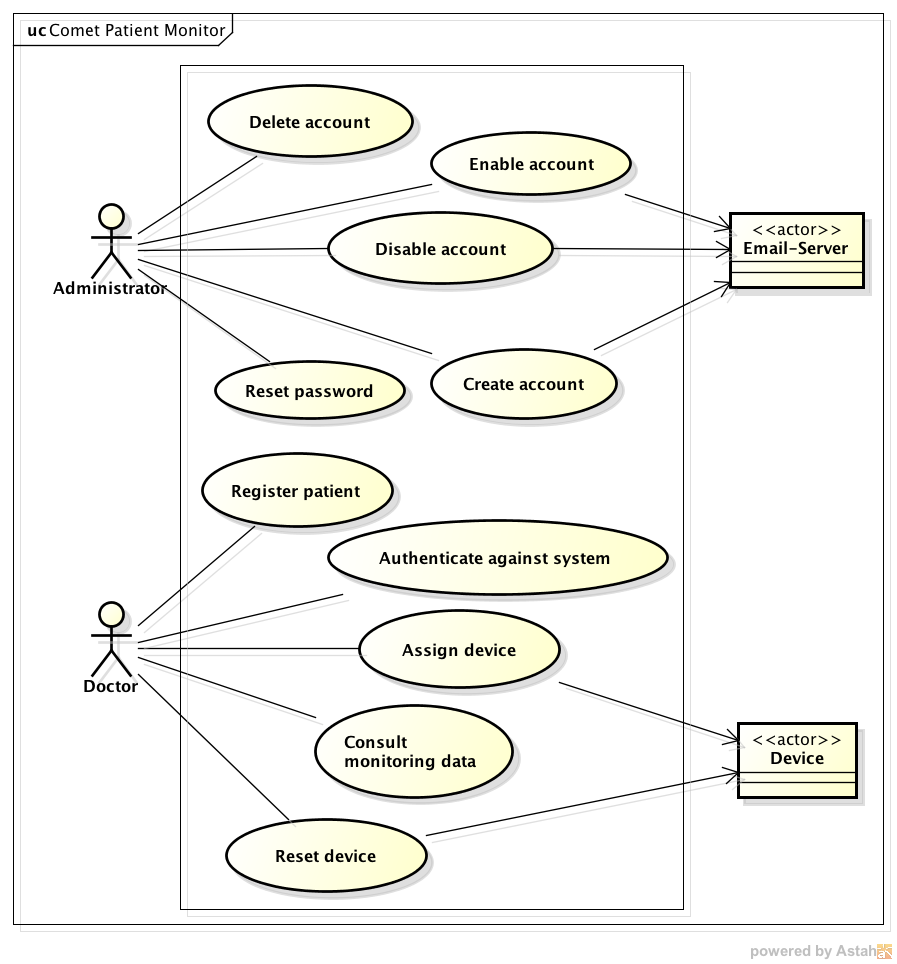
\includegraphics[width=15cm]{./use-case-diagram.png}

\end{document}